\section{Results} % (fold)
\label{sec:results}
    \subsection{Environment} % (fold)
    \label{sub:environment}
        When the web page containing the model loads, a recognisable representation of the University of Queensland's is visible.

        \begin{figure}[H]
            \centering
            \fbox{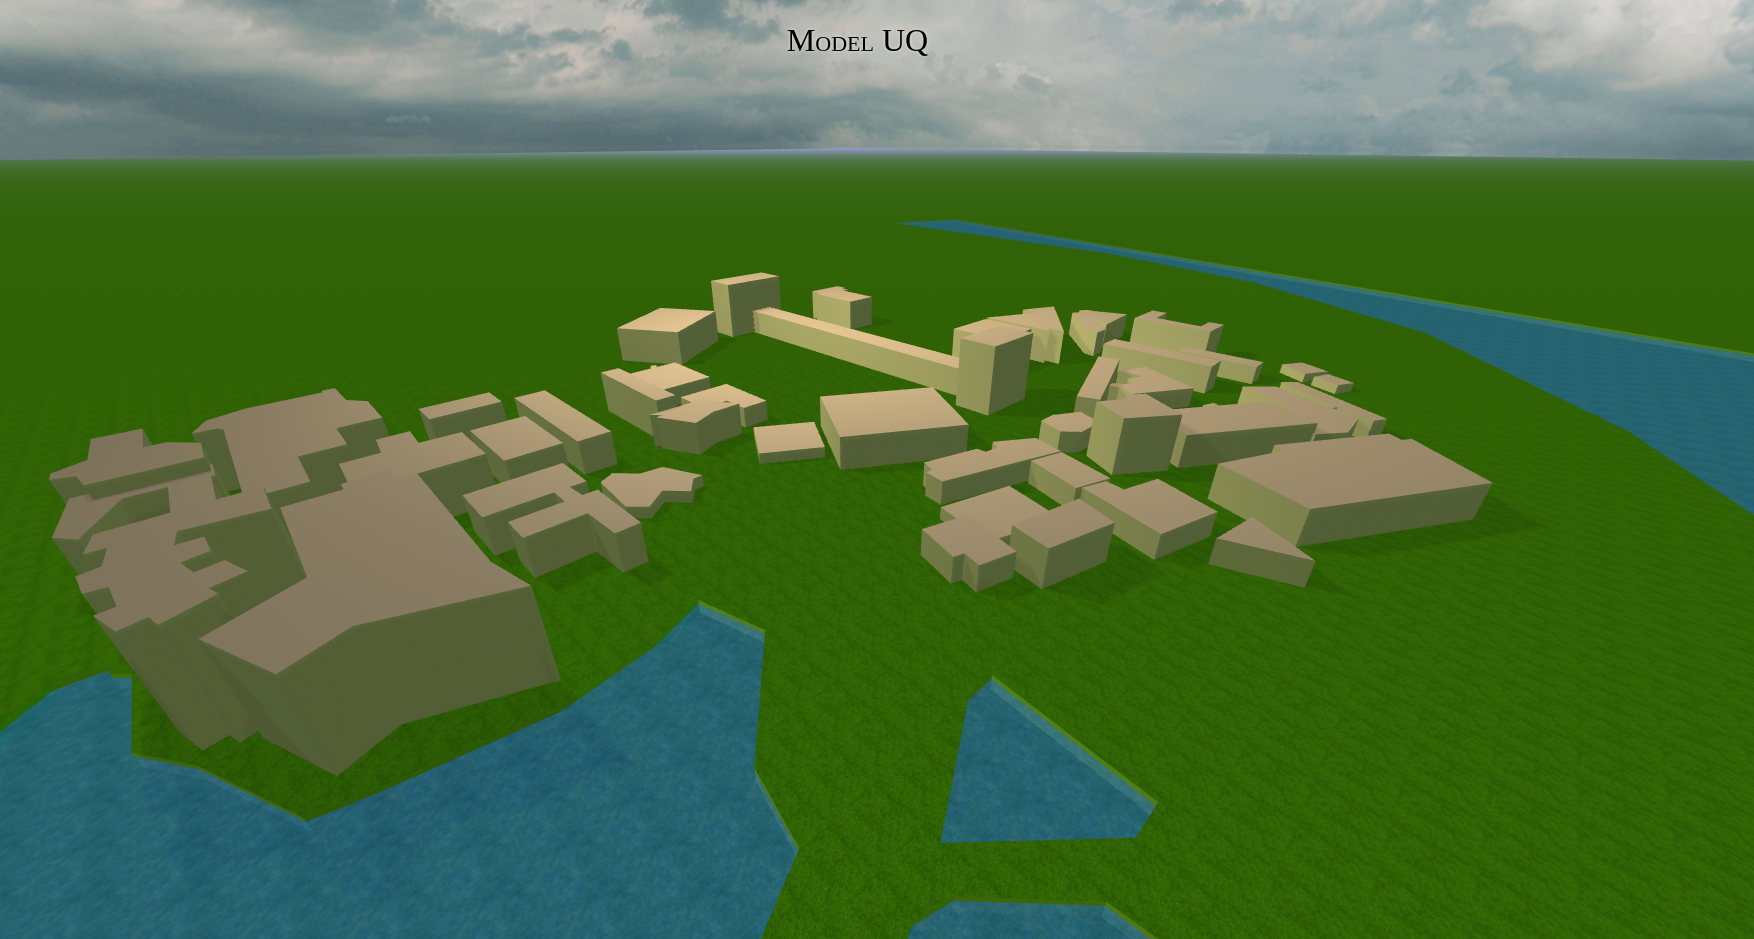
\includegraphics[width=\textwidth]{start}}
            \caption{
                Screenshot after the web page loads.
            }
            \label{fig:start}
        \end{figure}

        It is clear that there are many buildings in a location surrounded by
        a couple of bodies of water, including what appears to be a river wrapping around.
        Should the user be familiar with the St Lucia Campus, the Forgan Smith building and the Great Court are particularly recognisable as major features identifying the campus.
        Many of the structures are also immediately recognisable, such as the distinct wedge shape of the Advanced Engineering Building overlooking the lakes, and the Michie and Duhig tower buildings bookending the Forgan Smith.\\

        It is also evident the water bodies are recessed into the ground, with a defined depth, below the level of the water.
        The other major striking feature evident early on is the presence of a realistic sky, normally coloured and with clouds in the distance.\\

        Overall, the scene conveys an understandable representation of a set of buildings, with multiple bodies of water in the vicinity quite successfully.
        A user observing this model should be able to immediately get a sense of orientation and the positioning and heights of the buildings present.
    % subsection environment (end)

    \subsection{Texturing} % (fold)
    \label{sub:texturing}
        While reasonably subtle from long distances, it becomes much clearer upon inspection that the grass, buildings, and water are all textured (see figure Figure~\ref{fig:texture}).
        When zooming up on the surface of the buildings, the bump mapping used becomes very apparent, and produces a very believable and clear representation of sandstone bricks (see Figure~\ref{fig:bump_map}).

        \begin{figure}[H]
            \centering\fbox{
                \begin{subfigure}[t]{0.5\textwidth}
                    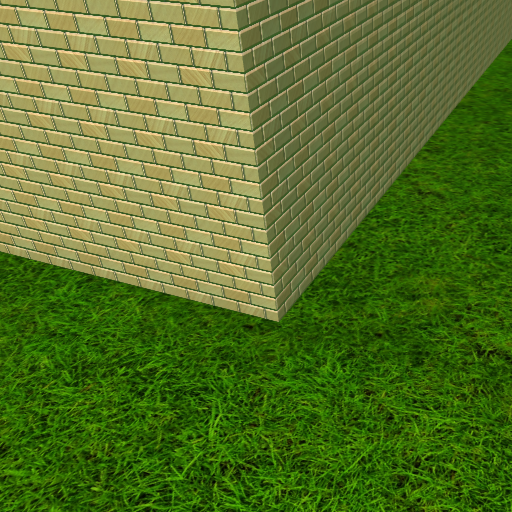
\includegraphics[width=\textwidth]{texturing}
                    \caption{Example of the sandstone and grass texturing.}
                    \label{fig:texture}
                \end{subfigure}
                ~
                \begin{subfigure}[t]{0.5\textwidth}
                    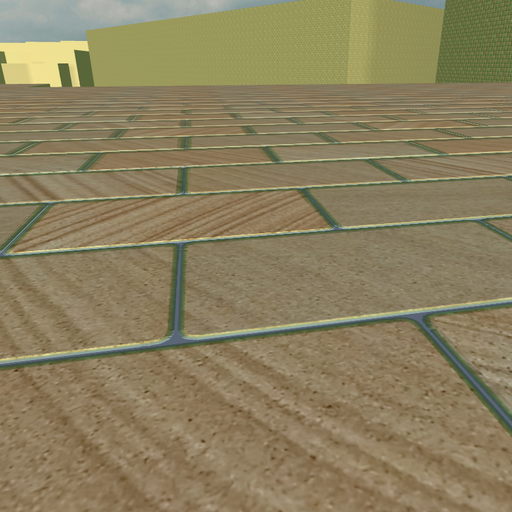
\includegraphics[width=\textwidth]{texture_and_bump}
                    \caption{Bump mapping in effect. Note the occluded edges of bricks further back.}
                    \label{fig:bump_map}
                \end{subfigure}
            }
            \caption{Texturing screenshots.}
            \label{fig:texture_examples}
        \end{figure}        
    % subsection texturing (end)

    \subsection{Lighting} % (fold)
    \label{sub:lighting}
        The lighting of the scene greatly improves the quality of the model.
        Having moving shadows, and correctly lit surfaces is very useful for the users depth perception and the believability of the model.

        If the scene is observed for even a small length of time, it becomes apparent that the shadows are moving around the buildings in a circular fashion, and also changing lengths.
        The shadows cast by the buildings definitely contribute to improving the quality of the scene.

        \begin{figure}[H]
            \centering
            \fbox{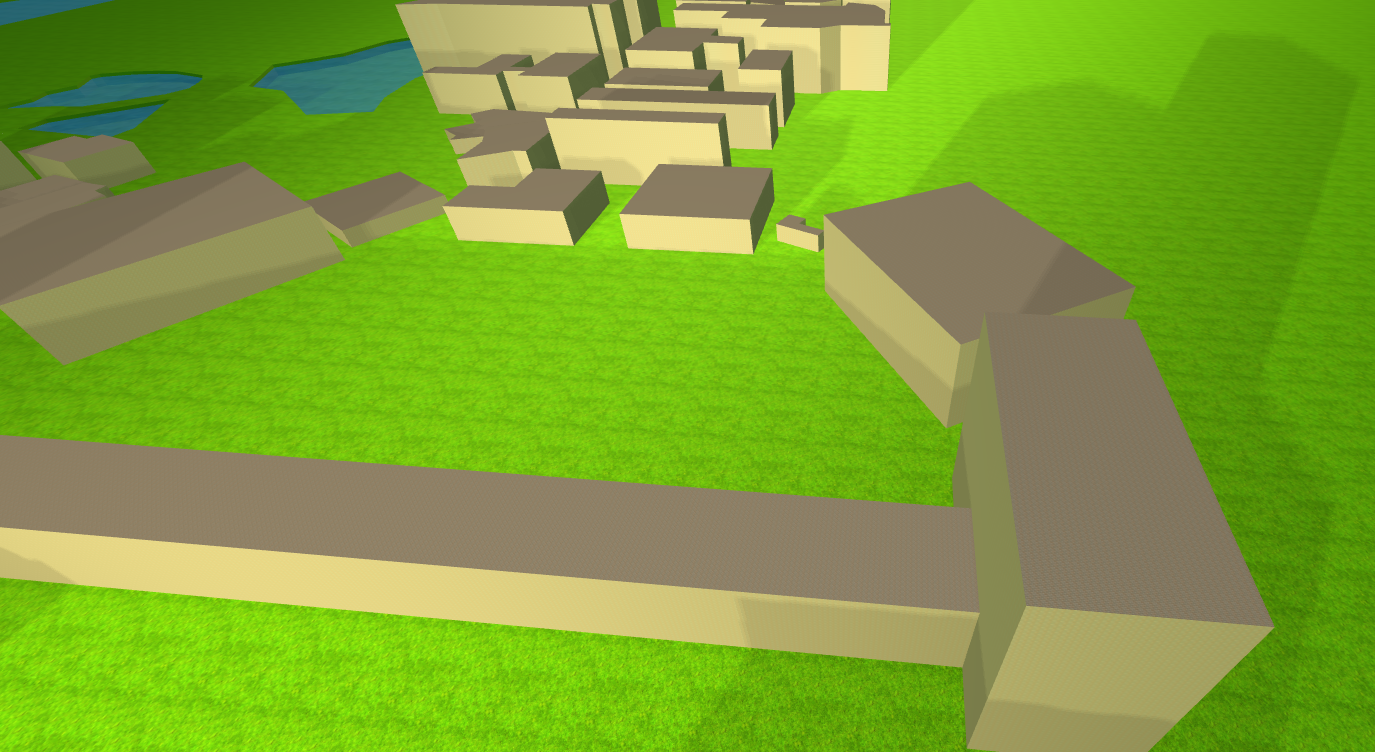
\includegraphics[width=\textwidth]{shadows}}
            \caption{
                Screenshot of shadows being cast by buildings around the great court, with the sun at a low angle.
            }
            \label{fig:shadows}
        \end{figure}

        A more subtle lighting phenomena is the simulation of a diffuse reflection from the grass onto the bump mapped bricks.
        This is caused by the hemispherical lighting used to simulate sunlight.
        What is seen is a

    % subsection lighting (end)
% section results (end)